\subsubsection{Stump volume}
\label{sec:allo}
First, $dbh$ is calculated from tree mass $M$
\begin{equation}
    \label{eqn:dbh}
    dbh=a*M^b
    \end{equation}where $a=0.122$ and $b=2.38$ from \cite{Landsberg1997}.
Then we calculate total tree height ($H$) using coefficients provided by \cite{Brahim2000}
\begin{equation}
    \label{eqn:height}
    \begin{bmatrix}\frac{14705.8823529412 M + 250.0 d^{2.34} -56617.6470588235}{D^{2.34}}\end{bmatrix}
    \end{equation}where $D$ is $dbh$ for the individual tree and $d$ is the stand average $dbh$. We the use of stand average can improve the accuracy of the relationship, however as the 3-PG model does not predict variation in $dbh$ between stands we simply use the derived $dbh$ from \ref{eqn:dbh} fro both values. \citeauthor{Benbrahim2003} also provides \ref{eqn:taper} to determine diameter at a given height or height at a given diameter:
\begin{equation}
    \label{eqn:taper}
    0=-d+\left(b_d-b_d\left(\frac{\log{\frac{1-h}{Ha}}}{-b}\right)^{1/c}\right)
    \end{equation}The taper equation provided by \citeauthor{Benbrahim2003} also requires a basal diameter ($b_d$). We calculate $b_d$ modifying equation \ref{eqn:taper} using coefficients provided and $H$, $dbh$ from above. Using a stump height of 10.0 cm we calculate the top stump diameter with whihc we can calculate the stump volume.
\begin{equation}
    \label{eqn:sectionvolume}
    V=\left(\frac{l\pi}{12}\right)(d_1^2+d_a^2+d_1d_2)
    \end{equation}We then calculate stump mass using a wood density of 0.38 $g \cdot cc^{-1}$ and compare with total tree mass $M$
\subsubsection{Stump volume regression}
To determine a simplified relationship between tree volume and stump volume we derive coefficients $a$ and $b$ in ~(\ref{eqn:form}) using a the ratio of stump mas to total stem mass over a range of stem volumes based on the allometric relationships in section \ref{sec:allo}.\begin{figure}[h]
     \centering
    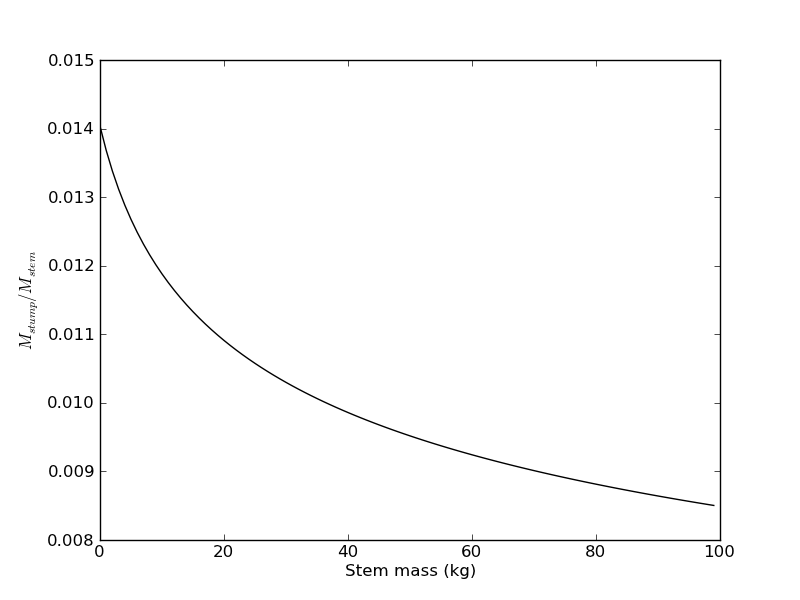
\includegraphics[width=0.5\textwidth]{nlm_stump.png}
    \caption{Stump to stem volume ratio as a functionof stem volume}
    \label{fig:stump_vol}
    \end{figure}
Coefficents used in calculating stump volume as a function of total stem volume were found to be $a=0.0179877356445$ and $b=-0.169054308617$.